% \documentclass[a4paper,10pt]{article}
\documentclass[twocolumn,a4paper,10pt]{article}
\usepackage{geometry}
\usepackage[T1]{fontenc}
\usepackage[utf8]{inputenc}
\usepackage{lmodern}
\usepackage[english]{babel}
\usepackage{url}
\usepackage{hyperref}
\usepackage{subcaption}
\usepackage{graphicx}
\usepackage{amsmath}

\geometry{a4paper,
 left=20mm,
 right=20mm,
 top=30mm,
 bottom=30mm,
}


% Training subcaption package to comply with
% IEEE standards. We can ignore the warning
% generated by caption.sty which is due to 
% the redefinition of \@makecaption
\DeclareCaptionLabelSeparator{periodspace}{.\quad}
\captionsetup{font=footnotesize,labelsep=periodspace,singlelinecheck=false}
\captionsetup[sub]{font=footnotesize,singlelinecheck=true}


\title{Machine Learning Homework 4:\\Markov Decision Processes}
\author{Nicolas Six}

\makeatother

\begin{document}
\maketitle \tableofcontents{}

%%%%%%%%%%%%%%%%%%%%%%%%%%%%%%%%%%%%%%%%%%%%%%%%%%%%%%%%%%%%%%%%%%%%%%%%%%%%%%%%%%%%%%%%%%%%%%%%%

\section{Introduction}

\paragraph{}

In this work we will explore solutions to solve problems that can
be described as Markov Decision Processes (MDP). This sort of problems
are very common and are generally found in games, but are not limited
to them as lot of real life problems can be represented by this kind
of approach. MDP is not always the best way to model a problem but
it is interesting enough to be, nowadays, at the heart of artificial
intelligence research. The goal of this report is not to present state
of the art method but more to gain experience from now classic techniques.

We will here start by applying two well known algorithms to find policies
for two given problems. We will then explore the possibility
to learn a policy directly from the problem, without needing any model
from it.

We will use in this report the same convention as previously concerning
plots. Unless stated otherwise, on each graphs, the hard line represent
the median value of all the experiments and the hue area cover the
space between min and max values.

\subsection{Problems}

\paragraph{}

During this assignment we will study two different problems, or more
exactly two different version of one famous problem. This MDP problem
is the case of an agent playing at Starcraft II. You probably remember
that our previous study were often grounded in Starcraft II, not that
it is a game we played, we just played one or two games to try it. If
we were so interested in Starcraft II, it is because of an other project
we started last semester with a group of friend to try to build an
AI for Starcraft II using RL among other things. We will build our
work here around it, and try to show some interesting aspect of this
problem.

Since Deepmind created an AI capable of winning against the bests
Go players in the world \cite{AlphaGo0}, Starcraft II is often referred
as the new challenge for artificial intelligence. This game is very
interesting in an AI point of view as it mix together global strategy
to defeat the enemy with low level micromanagement as well as a complex
balancing system allowing a great number of possibilities. In addition,
the number of possible state in this game far bigger than the one
of Go and the action space is quite impressive too, the effect of
the chosen action often have no direct impact and an agent must then
wait a long time to get the reward of the action it chose. This special
combination of very short term reward and very long term one make
that problem very challenging and let suppose plenty of real life
application for the techniques developed to build this first step
toward general artificial intelligence. This is why this problem is
not only investigated by lot of research team in the public field
but also by companies such as Google's Deepmind or Facebook research
lead by Yann LeCun. A lot of bot contest for Starcraft already exist,
but even the best bot of this competitions have no chance to win against
moderate level human player, showing that this question remain open.

To allow the development of new bots, Blizzard (the Starcraft creator)
and Deepmind released last summer an API, pysc2, that make the development
of RL bots easier in Starcraft II. Among other things this API let
us run the game on Linux without the GUI, allowing to run a full 20
minutes games in a couple of minutes. It may look fast but RL methods
need a lot of examples, and some minutes are enough to transform learning
session in hours.

As already stated above with a group of friends we used this API to
build an artificial intelligence. Our goal was to build a general
structure of multiple agent working together to build the whole AI.
This approach is the one used in most of the actual bots, but is not
the one presented by Deepmind in the paper accompanying the release
of pysc2. Our goal is to cut the difficulty of the game into smaller
problem that classic RL methods can solve. This project, which we
named \href{https://github.com/Xaxetrov/OSCAR}{OSCAR}, is still ongoing
and is far from beating any common bot at this point, but provide
a good ground to build our experience for this work.

OSCAR also gave a set of meta action allowing to build small chain
of action to achieve a given task. For example, to build a barrack
in Starcraft II, you need to select a worker and ask him to build
a barrack in a free position available on the screen. A meta action
will do the same sequence of action in the game point of view but
will make it simpler for the agent, as it will not have to chose which
worker select and were the barrack will be build.

In the learning point of view one of the advantage of OSCAR here is
that it made all the structure available as an openAI Gym environment.
It is then easy to plug into most of the available reinforcement learning
algorithm available on the web. From this we build two specific environment
trying to tackle the same problem, beat an original Starcraft AI on
a very basic map.

The reward we chose are the same for both problems. A reward of 1.0
is given for a victory and 0.0 for a defeat, as the games are bounded
in time, we also set a reward of 0.2 when no player win. We added
to that some rewards to make our agent more offensive. We set a reward
of 0.1 for killing at least an enemy unit in the last step and 0.2
for a building as well as a reward of 0.1 for creating a marine.

\subsubsection{Basic version}

\label{basicVersion} 

\paragraph{}

The first version of the problem we will use here is pretty basic.
The goal of this environment is to be the simplest possible while still
allowing the AI to build an army and hopefully win.

The state we chose is a set of five boolean values, totaling 32 different
possibilities. This state is composed of the information if at least
a supply depot have been built (required to build a barrack), if at
least a barrack have been built, if we have reached max population,
if we have at least 10 soldiers and finally if the enemy base position
is known. In the action point of view, we also selected very basic
ones. The five meta action we chose are build a supply depot, build
a barrack, train a marine (basic soldier), select the army and attack and lastly
do nothing. You can see that this set of action / state is very different
from playing the full game, but will allow to build some soldiers
and attack the enemy in a very basic fashion. A human playing this
game will probably not enjoy it, as it will be like having five led
in front of him and five possible button to use, with the additional
difficulty for an agent that it does not have any memory in addition
to the one provided by the five leds.

The main advantage of this version is to be very basic. With only
32 states and 5 actions, it will demonstrate the possibilities of
classical approach to RL, and display their advantages.

\subsubsection{Complex version}

\paragraph{}

The second version of our environment is a bit more complex. This
problem not as basic as the previous one and allow the agent to have
a better understanding of its state, but with few difference in terms
of actions.

In this case the state is far bigger, with 2~982~525 different state
possible. The main difference here is that the values are not boolean
anymore but can take multiple values. In comparison to the basic version,
the state now give the number of supply depot build in the range 0
to 22, the number of barrack from 0 to 4, the size of the army from
0 to 180 with step of 10, the number of worker collecting resources
from 12 to 24 and an information on the time spend on this game simplified
on 5 different steps. In terms of action this version has exactly
the same than the one described in section \ref{basicVersion}, with
the notable addition of an action to create new worker.

This version add a lot more possibilities, as for example basic economic
management and far more information on the current game. This added
information will allow a deterministic agent to build more complex
strategies, but will also make it difficult to explore all the different
possibilities. If this was designed to keep this number small enough
to make value iteration possible, it will exhibit some of the limit
of the classical approach which are value iteration and policy iteration.

\section{Solving MDP}

\subsection{Introduction}

\paragraph{}

A good way to find a good policy in a MDP context is to
ether use value iteration or policy iteration, both of them will hopefully
converge toward optimal policies. The problem of such algorithm is
that they must know the entire set of possible state, transition and
the underling reward and probabilities. It's probably not a problem
in most of toys game used as example in reinforcement learning, but
can become much more problematic in the case of POMDP, of which games
such as Starcraft are good example as the state of the enemy is mostly
unknown by the agent.

To counter that problem and the fact that we do not have directly
access to the state and transition of our problems, we decided to
create a basic model of them. Those models take a lot of different
assumption on the game and are not perfect representation of it. Due
to this approximations, if we will fund polities that are optimal
for our simplified version they will not be for the real environment.

The main assumption we made in our simplified environment is that
each action as a direct effect on the state. For example, asking for
training a marine give you one in the next state as well as attacking
the enemy which directly in the next step kill all your army but may
get you some rewards. Reward is also the major difference between
the two problems. The basic one get the same reward when it attack
with ten marines at the start of the game or at the end, because it
as no idea of how long the game was, while in reality attacking with
ten marines at end of game usually do very little damage to the enemy.
That's also why we added a notion of time the complex version and
simulated the grow of an enemy army.

An other approximation we made is that the enemy never attack, and
so that you only lose our army when you attack and can not lose that
game, which is not really a problem here as we defined a lost game
as a null reward, the same as most of the possible actions.

This approximations of the environments can be viewed as domain knowledge,
as they transform the game and rate it in a way that is personal to
us. The way the probability of the transition is, for example, something
that only an expert can do correctly. We tried here, with our modest
experience in the game, to be as close as possible to the original
environment, with our constraint on the state. This domain knowledge
exhibit the fact that the result directly come from the rules given
by an expert of the domain, which probably build them with a policy in
mind.

\subsection{Value Iteration}

\label{vi} 

\paragraph{}

Value iteration is the most stretch forward way to get a good
policy from a perfect knowledge of transitions. We will try here to
asses its results, particularly regarding the number of iteration
needed to converge toward a policy.

\begin{figure}
\centering \begin{subfigure}[t]{0.7\columnwidth} \centering
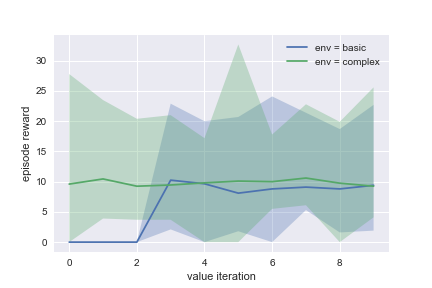
\includegraphics[width=1.1\linewidth]{{../graphs/all_value_iteration_episode_reward_env}.png}
\caption{Reward get by the agent according to the iteration}
\label{fig:vi_reward} \end{subfigure} \begin{subfigure}[t]{0.7\columnwidth}
\centering 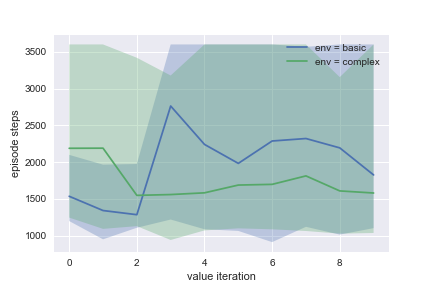
\includegraphics[width=1.1\linewidth]{{../graphs/all_value_iteration_episode_steps_env}.png}
\caption{Duration of a game in steps, according to the iteration}
\label{fig:vi_steps} \end{subfigure} \begin{subfigure}[t]{0.7\columnwidth}
\centering 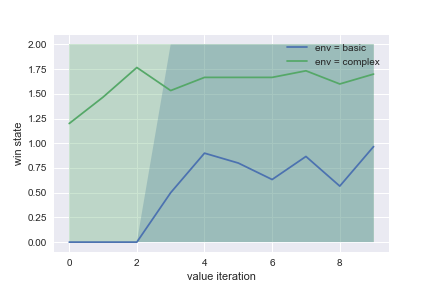
\includegraphics[width=1.1\linewidth]{{../graphs/all_value_iteration_win_state_env}.png}
\caption{Victory / defeat state at end of game according to the iteration.
0 is defeat, 1 null and 2 victory. The hard line represent here the
mean value (and not the median as in other Figures)}
\label{fig:vi_win} \end{subfigure} \caption{Progress of the agent with the iteration of value algorithm}
\label{fig:vi} 
\end{figure}

Figure \ref{fig:vi} show the agent results when using the policy
get at a given iteration. For this set of test, we used a learning
rate of 0.1 in both case without setting a $\Delta$ limit as we wanted
the algorithm to try to improve the policy at each steps. We will
study more in depth the effect of those parameters later on the is
section.

You can see on Figure \ref{fig:vi_reward} that environment converge
toward similar results, which we must admit surprised us as we were
expecting the basic environment to be too simple to get correct results.
However, we can note that the complex version get correct result as
soon as the first iteration and then change very slowly. In addition
if we know that the basic version converge in the fourth iteration
the complex version does not converge before the $19^{th}$ and still update
its policy for about 7000 actions on the five last step of this graph.
Even if this is very small in comparison to the $3\cdot10^{6}$ state
possible, particularly if you consider that most of this states are
not possible in the game, it is still not negligible. However, this
update are probably minor as they did not results into reward variation
bigger than the underling noise we can observe on the basic case from
iteration 3.

If you combine the results of Figures \ref{fig:vi_steps} and \ref{fig:vi_win},
you can see that, first the basic version lose quite quickly it's
games and then converge to a policy allowing it to win some of its
game, but mostly staying alive long enough to prevent loosing. While
the complex version is more trying to end the game as quickly as possible,
winning most of the time but not every times.

As we already stated previously the complexity of the environment
have a big effect in terms of convergence toward a stable policy,
but the variation are very small after the first iterations. Thus
value iteration seams to be able to find good policy in few iterations,
it was able to converge after three iterations on the basic problem.
But if the complex problem gave good results since the first iterations,
it takes 19 of them the reach a stable state.

\begin{figure}
\centering \begin{subfigure}[t]{0.7\columnwidth} \centering
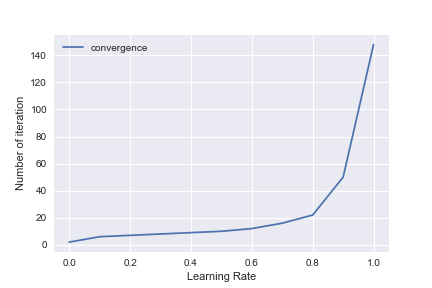
\includegraphics[width=1.1\linewidth]{{../graphs/value_gamma_iter}.png}
\caption{Evolution of number of iterations to convergence according to gamma
value for delta of $10^{-}8$ (delta of policy evaluation)}
\label{fig:vi_param_gamma} \end{subfigure} \begin{subfigure}[t]{0.7\columnwidth}
\centering 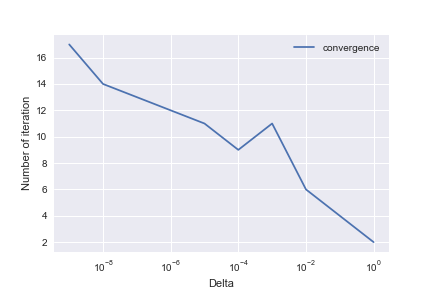
\includegraphics[width=1.1\linewidth]{{../graphs/value_delta_iter}.png}
\caption{Evolution of the number of iterations to convergence according to
the delta value used for policy evaluation, with a gamma value set
to 0.5}
\label{fig:vi_param_delta} \end{subfigure} \caption{Effect of the different of the different policy parameters on the
convergence time}
\label{fig:vi_param} 
\end{figure}

\paragraph{}

You can see on Figure \ref{fig:vi_param} the effect of the two main
parameters of value iteration. We run this exploration only on the
basic problem because as the complex problem's transition table does
not fit into our RAM it will have taken days to do the same for this
problem. It is easy to show that doing so will only give us similar
results with larger convergence time as the two problems are very
similar, the only difference being the number of states. The policy
find was the same in every cases explored here. Apart from the cases
when $\gamma=0.0$ and $\gamma=1.0$, where the policy was completely
suboptimal because of horizons problems.

As you can see on Figure \ref{fig:vi_param_gamma}, in our case, the
smaller $\gamma$ is the faster we get to the results. However, taking
too small $\gamma$ values will quickly led to horizon problems. We
suppose then that if relatively small values still work here it is
because the optimal solution does not follow a very long path. But
also because our transitions has a very small stochastic component.
Thus we suppose that taking large $\gamma$ is more robust to complex
problems but at the cost of computation time.

Considering the stopping condition, the number of steps appear to be
correlated to the log of the desired $\Delta$ between the value of
two iterations. This result is displayed on Figure \ref{fig:vi_param_delta}.
This is a good news as you can expect to get better results at minimal
cost. However, we got here the same results every time, showing that
our problem is simple enough to be solved in a very small number of
iteration. You can note an outlier on graph for $\Delta=10^{-3}$,
the only explanation we manage to find for it is related to the random
value we use as a starting point.

\subsection{Policy Iteration}

\label{pi} 

\paragraph{}

Policy iteration is very similar to value iteration, particularly
when looking for an optimal policy. This similarity is particularly
important in terms of results as both of them converge toward mostly
identical policies.

We will here perform a similar study as in the previous section to
see the impact of each iteration in terms of reward in the actual
game as well as win / loss proportions and game duration.

\begin{figure}
\centering \begin{subfigure}[t]{0.7\columnwidth} \centering
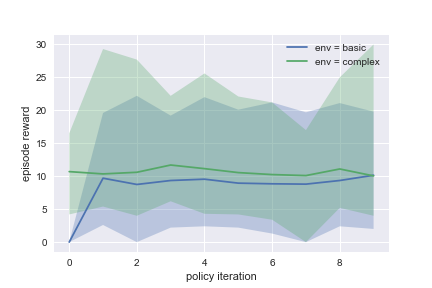
\includegraphics[width=1.1\linewidth]{{../graphs/all_policy_iteration_episode_reward_env}.png}
\caption{Reward get by the agent according to the iteration}
\label{fig:pi_reward} \end{subfigure} \begin{subfigure}[t]{0.7\columnwidth}
\centering 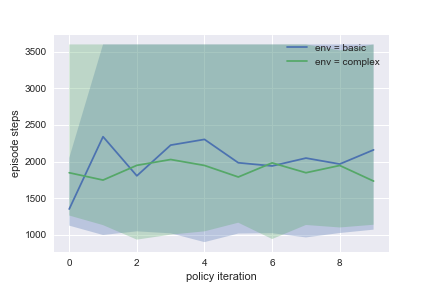
\includegraphics[width=1.1\linewidth]{{../graphs/all_policy_iteration_episode_steps_env}.png}
\caption{Duration of a game in steps, according to the iteration}
\label{fig:pi_steps} \end{subfigure} \begin{subfigure}[t]{0.7\columnwidth}
\centering 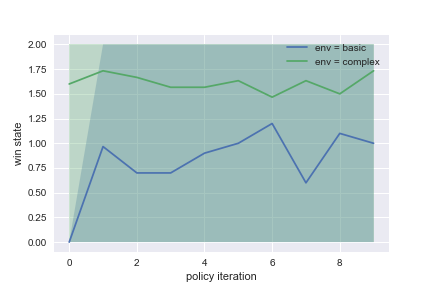
\includegraphics[width=1.1\linewidth]{{../graphs/all_policy_iteration_win_state_env}.png}
\caption{Victory / defeat state at end of game according to the iteration.
0 is defeat, 1 null and 2 victory. The hard line represent here the
mean value (and not the median as in other Figures)}
\label{fig:pi_win} \end{subfigure} \caption{Progress of the agent with the iteration of policy algorithm}
\label{fig:pi} 
\end{figure}

As you can see on Figure \ref{fig:pi}, both problems get some what similar
results. As with value iteration the complex version get better results
than the basic, while both of them are trying to solve the same problem,
but with different tools.

On a general basis, both environment converge toward a stable policy
in about two iterations, the variation are seen on the plot after
this iteration are only due to the random aspect of the environment
and the approximation made to construct the policy. To give precise
numbers, the basic version converge at the second iteration
while the complex problem it converges at the fifth step, but already
have a very good approximation of this final policy at the second
one.

On Figure \ref{fig:pi_reward}, you can see that the complex environment
get high reward as soon as the first iteration. We did not expected
it to converge that soon. Our supposition to explain that as it has
far more states, the first iteration see enough transitions to compute coherent
policy. We can not also exclude the possibility of chance as we start
with a random policy but given the number of state, it is quite unlikely.
The basic version get bad results here, with a median reward being
about half the one of the complex version. In addition we must note
that it take longer to train it in terms of iteration as it have to
wait the second iteration to see improvement in terms of reward.

In game duration point of view, Figure \ref{fig:pi_steps} show that
the complex version manage to run the game during shorter times. It
worth mentioning that if you merge this results with the one of Figure
\ref{fig:pi_win}, not only the complex environment make the games
finish sooner but it also win a lot of them, whereas the basic environment
only lose most of them, and sometime manage, by chance, to win one.
Showing again that optimizing our reward allow the agent to find a
coherent policy for the real environment. If such a policy is not
always enough to win, as in the case of the basic problem, you can
still note the link between reward and win / defeat, but also that this link does not hold in both directions, an agent winning most of its game does not get necessarily better result than one which do not win.

We can note here that the complexity in the dimentionnality of state
space make the convergence a little longer. If the basic version converge
in the second iteration, the complex version converge in the fifth.
Considering that the complex environment as more than 90~000 time
the number of state of the basic one, we can see that as a minor cost.
Even if it must be noted that the iteration in the complex case are
far longer than in the basic one.

\begin{figure}
\centering \begin{subfigure}[t]{0.7\columnwidth} \centering
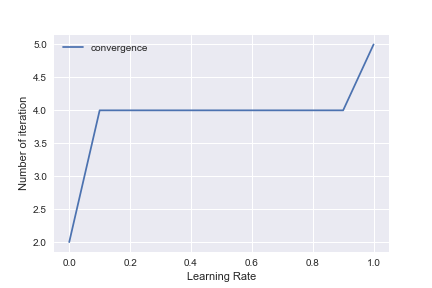
\includegraphics[width=1.1\linewidth]{{../graphs/policy_gamma_iter}.png}
\caption{Evolution of number of iterations to convergence according to gamma
value for delta of $10^{-}8$ (delta of policy evaluation)}
\label{fig:pi_param_gamma} \end{subfigure} \begin{subfigure}[t]{0.7\columnwidth}
\centering 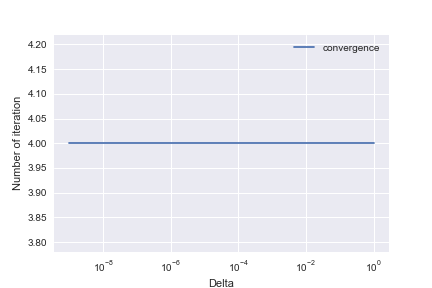
\includegraphics[width=1.1\linewidth]{{../graphs/policy_delta_iter}.png}
\caption{Evolution of the number of iterations to convergence according to
the delta value used for policy evaluation, with a gamma value set
to 0.5}
\label{fig:pi_param_delta} \end{subfigure} \caption{Effect of the different of the different policy parameters on the
convergence time}
\label{fig:pi_param} 
\end{figure}

\paragraph{}

Policy iteration is quite stable when regarding the effect of its
different parameters on convergence time. We explored on Figure \ref{fig:pi_param}
the effect of them on the basic problem only, because as the transition
table do not hold in RAM for the complex one, the process will have
taken days on this last problem, just to get similar results.

As we said previously this algorithm is very stable, we did not fund
any parameters that managed to change the time need to make it converge.
Apart from the particular case of $\gamma=0.0$ and $\gamma=1.0$
where both the policy and the iteration number became
meaning less due to horizon problems. In all the other cases policy
iteration converge toward the same policy into four iterations no
mater $\gamma$ value or the precision of the policy value estimation.

\subsection{Conclusion}

%why we didn't discussed wall time... (disk / ram)
% compare policy of the two methods
% compare speed
% param effect: not so stocastic env
% same resutls (testes on basic)

In conclusion, the two algorithms explored here do a good job in those
cases. Both of them end up giving the same policy on the basic problem,
this is not really the case for the complex problem, where after 20
iterations value iteration converge to a policy where 3~936 actions
are still different from the policy get by policy iteration. However,
this only represent 0.13\% of difference in the policy, knowing that
most of the state are probably possible but never appear on real game.
At the end of the day, those two policies are very similar.

We must also note that in both case the link between reward and victory
is not that clear, and good rewards be achieved without winning. This
show that our reward definition is not perfect need some adjustment
to let the agents win more games. Such a change that we will have
tried given more time is to only use the final game reward as the
only possible reward.

The main difference between them is the time needed to converge. Value
Iteration can take a lot of iterations to give it's results as we
showed on section \ref{vi}. However, those additional iteration did
not change the final policy in our particular case. This is the reason
why policy iteration finish in less iteration as it stop when policy
do not evolve no matter if the underling value is exactly the one
of the problem or not. If policy iteration is faster regarding the
number of iterations it is not necessary the case in terms of wall
time. For example, when the cost of reading the transition table is
important, then evaluating the utility of a policy cost nearly the
same as running value iteration. This was our case for the complex
problem where the transition table must be written to disk.

When building the simplified version of the two problems to generate
the transition table, we unconsciously reduced drastically the stochastic
aspect of our problems. Making it easier to generate but also to learn
from. This can be clearly seen through our parameters study as the
policy remained correct with most of the parameters. If it difficult
to be sure due to the noise of our results, we also suppose that the
decreasing tendency you can see on both Figures \ref{fig:vi_reward}
and \ref{fig:pi_reward} is due to an overfit of the policy to our
model of the problem.

That two lasts points show us the limits of the techniques used here.
If they work remarkably well, they need a perfect knowledge of the
environment. Such knowledge is often really difficult to get from
real system, in other case it often is too large to be usable and
most of all it is often biased by the people constructing the model.
If we can discuss the usefulness of such a bias it is sometimes interesting
to be able to learn without being constraint by the dogmatic knowledges.

\section{Dueling Q-Learning}

\subsection{Introduction}

\paragraph{}

The method we choose to use here is a particular version of the Q-learning
algorithm witch was first presented by Wang et al. (2016) \cite{DuelingQL}.
The original version is presented as part of Deep Q Network (DQN)
but deep part of the network is mandatory.

We chosen to use for both problem a basic network build around three
dense hidden layers of sixteen neurones each. While this structure
stay very basic, it is probably complex enough to handle the complexity
of both environments. State of the art methods manage to learn policies
above the human level in days, as we plan here to test different set
of parameters such training time is not conceivable. Even we can argue
that our problem are far more simple than learning Atari game from
pixels the time needed to generate the examples and the number of
test we want to run, make time one of the biggest constraint here.
Thus we decided to run our test on 100~000 steps, which is equivalent
to 60 to 80 full games depending on the length of the games.

\subsection{Basic Idea of the algorithm}

\paragraph{}

A dueling network is very close to a classic Q-Learning network in
the way that both of them take the state as input and output the state-action
value $Q$. The particularity of the Dueling network is that instead
of learning directly this $Q$ value for each state action pair, it
decompose it as two different things, as you can see on Figure \ref{fig:DuelingDQN}.
First the state value $V(s)$ which give the value of the current
state. Second the advantage representing the benefit of taking a given
action when in the current state, $A(s,a)$. This component are then
simply used to compute the $Q$ value using the following equation:
\[
Q(s,a)=V(s)+A(s,a)
\]

The benefit of this method is that the advantage is the same for all
the action of a given state. This particularity allow the network
to learn more easily that some state are good or bad no matter the
action you chose, reducing the number of samples needed to learn a
correct policy.

The other details on this architecture are out of scope here, but
we recommend the interested reader to report to the original paper
\cite{DuelingQL} for more precision on the implementation as well
as experimental result on Atari games.

\begin{figure}
\centering{}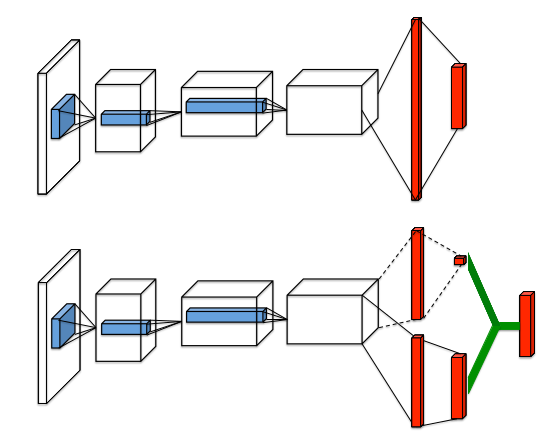
\includegraphics[width=0.8\linewidth]{duelingDQN} \caption{Dueling architecture as presented in \cite{DuelingQL}. Top network
represent the classic DQN structure while the bottom one represent
the Dueling structure}
\label{fig:DuelingDQN} 
\end{figure}

\subsection{Experiments}

\paragraph{}

Our experiment where produced using the algorithms provided by \href{https://github.com/keras-rl/keras-rl}{keras-rl}.
But before to present our results, we need to clarify some implementation
details.

First, the Q-Learning algorithm rely on a memory to remember the lasts
observed transitions. This memory prevent the agent to overfit in
the current state of the game and still have some examples of the
experiences of previous games. We chose to set such a memory for the
last 50~000 steps, which is more than 30 games. There are two different
strategy to fill this memory before learning anything. The first is
to play random action until the memory is filled and hope to have
a correct representation of the states. The second is to fill it with
examples and hope that the network will learn to copy them. The problem
of this last case is that examples are not that easy to find in most
case. Luckily, we have, tanks to the previous section, two agents
that perform correctly for both problems. To have a better idea of
the effect of such change in the train we explored the three different
possibilities: empty memory (overfit on the firsts observations), random
action memory and pretrained agent memory.

Second, as every reinforcement learning algorithm, Q-learning is subject
to the exploration / exploitation dilemma. To try to mitigate its effect here
we chose the following approach. We used a Botlzmann policy witch
make all action possible even if some of them may have very small
occurrence probability. We also increased this effect by setting the
temperature parameter to high value in the first iteration and decreasing
it toward 1.0 on a given number of step. Again we chose here to explore
different value for this parameter.

\paragraph{}

As you can see on Figure \ref{fig:dqn_ml}, the method used to fill
the memory as no apparent impact on the reward the agent get from
an episode. This showed to our surprise that the agent does not take advantage
of the experience we gave him. It really surprised us, as a paper
from Cruz Jr et al. \cite{DQNpretraining} showed exactly the opposite
result. This result also appear on Figure \ref{fig:dqn_ep_ml}, where
you can see that the noise as more importance here than this parameter.
Thus, this kind of exploration strategy does not give the results
we were looking for. Maybe a bigger memory and a longer training time
will have given different results but we were not capable of producing
such experiments.

\begin{figure}
\centering{}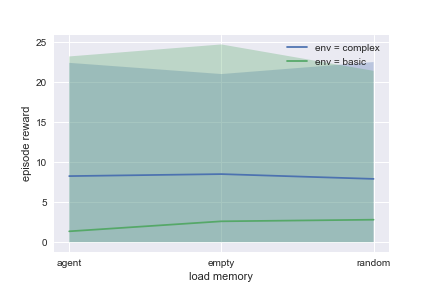
\includegraphics[width=0.8\linewidth]{{../graphs/dqn_load_memory_episode_reward_env}.png}
\caption{Evolution of the episode reward according to the method used to allocate
memory. Agent mean that the memory was filled with experience from
the previous section's agents, empty mean that nothing was stored
in it, random mean that first random action were chosen in order to
fill the memory.}
\label{fig:dqn_ml} 
\end{figure}

\begin{figure}
\centering{}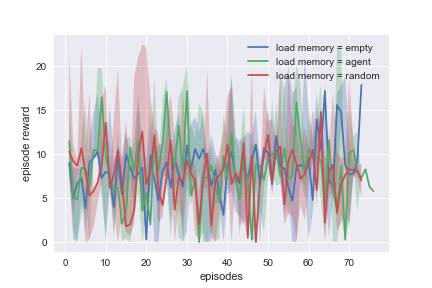
\includegraphics[width=0.8\linewidth]{{../graphs/dqn_episodes_episode_reward_load_memory_complex}.png}
\caption{Evolution of the episode reward according to the episode number during
training for different ways to fill replay memory.}
\label{fig:dqn_ep_ml} 
\end{figure}

\paragraph{}

The number of step set for the exploration part of the training also
showed very little importance in the final result. As displayed on
Figure \ref{fig:dqn_em}, this parameter appear to have no impact
on the complex environment. However, we can see a variation of the
maximum observed for the basic version. Figure \ref{fig:dqn_em_bs},
show more details on that point. You can see that while empty memory take
advantage of the longer exploration, agent memory usefulness completely
disappear with long exploration.

\begin{figure}
\centering{}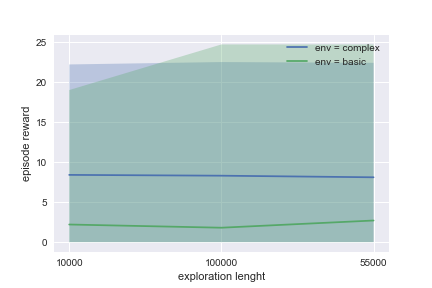
\includegraphics[width=0.8\linewidth]{{../graphs/dqn_exploration_lenght_episode_reward_env}.png}
\caption{Evolution of the episode reward according to the number of step spend
in linearly decreasing exploration mode.}
\label{fig:dqn_em} 
\end{figure}

\begin{figure}
\centering{}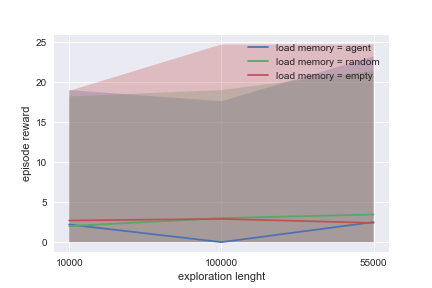
\includegraphics[width=0.8\linewidth]{{../graphs/dqn_exploration_lenght_episode_reward_load_memory_basic}.png}
\caption{Evolution of the episode reward according to the number of step spend
in linearly decreasing exploration mode for different memory allocation
on basic environment.}
\label{fig:dqn_em_bs} 
\end{figure}

\paragraph{}

On more general basis, you can see on Figure \ref{fig:dqn_rw} that
even if the result are noisy the learning agent managed to get a similar
reward than the agent using the policy produced by value iteration
or policy iteration. However, those result are not generalizable to
the basic environment where the reward is far lower than the one observed
previously.

\begin{figure}
\centering{}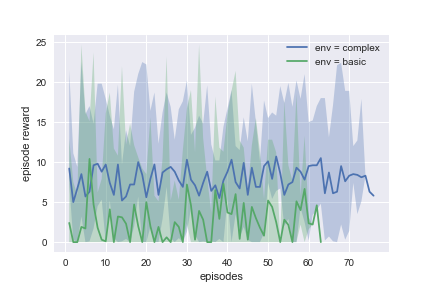
\includegraphics[width=0.8\linewidth]{{../graphs/dqn_episodes_episode_reward_env}.png}
\caption{Evolution of the episode reward according to the episodes for both
problems.}
\label{fig:dqn_rw} 
\end{figure}

\subsection{Discussions}

\paragraph{}

In conclusion, we can say that the results get in this section are
not as good as the one we get in sections \ref{vi} and \ref{pi}.
This is not really surprising as the informations given here are close
to none. The domain knowledge greatly improve the quality of the result
we get here and is the main difference between the two sections. In
the first case we determined a policy uniquely from domain knowledge,
never looking at the real system before to try our policy. In the
second case we never looked for domain knowledge and only interacted
with the environment to try to find something useful. We tried to
build a bridge between the two methods by filling the replay memory
with good example generated from domain knowledge, but it did not
give the boost we were expecting.

As said previously we were not targeting state of the art method and
so are convinced that RL can achieve far better results here. Such
improvement can come from different factors, such as the description
of the state given to the neural network. The learning algorithm used
can also make a big difference such as illustrated in \cite{A3C}.
In addition with a large number of state as we have here it probably
make sens to run the training on more steps. The 100~000 steps we
used here, takes about two hours to run but are still more than an
order of magnitude lower than the number of possible states. Some
reflection can also be done around the reward as it as been shown
that the this reward definition is not maximized when the agent win.
We can imagine an agent which as learned to keep his enemy alive to
be able kill more of its units and buildings, which will not help
him to win. At the same time, the rewards were designed to make the
learning process easier for RL by giving it middle ground steps.

We also never discussed the fact that if the agent always play with
the terran race, the enemy can be any of the three possible race:
terran, zerg and protos. This races being very different from one
to the other in terms of defense as well as in attack adding hidden
parameters in the state.

\section{Conclusion}

\paragraph{}

During this work we explored different ways to find good policies
when dealing with MDP. We first experimented with algorithms such
as value iteration and policy iteration, and discovered that they
managed to get good solution with relatively small need of computational
time. But we also approached their limits, in terms of complexity
due to the limited capability of a computer as well as in knowledge,
as it is not always possible to have perfect understanding
of the problem which this method require.

In the second part we found that RL can overcome this two difficulties,
with the example of a dueling Q-network. But if RL can pass those
difficulties, it come with a cost, the one of being able to get a
lot of example from the problems, if it is possible to do so with
a small memory foot print it usually require lot of computation time.
This time is manageable when you are dealing with computer generated
experiment, but when the process involve a human being or any real
world experiment such approach are too slow at current state of science.

We must admit that we wanted to use Asynchronous Advantage Actor Critic
\cite{A3C} instead of Q-network, but we did not manage to get a working
implementation of this method on our problems. If A3C is not the state
of the art any more, it is still a large step above the DQN on which
our work is based.

Our goal here was to gain as much experience as possible on MDP as
well as on classic RL methods. We only regret that we did not have
more time to go more in depth and try other modifications to both
the problems and the algorithms and hope to have more time available
soon to continue on this way.

You may have understood that we are particularly interested in that
field, but we still tried to answer the questions given in the description
and not only our own, as in the previous assignment. We tried here
to mix both point of view to provide interesting information for the
reader as well as valuable experience for us.


\bibliographystyle{plain}
\bibliography{rl}

\end{document}
